\documentclass[border=2mm]{standalone}
\usepackage{tikz}
\usetikzlibrary{decorations.pathreplacing}
\begin{document}
	%\begin{figure}[h!]
	%\centering
	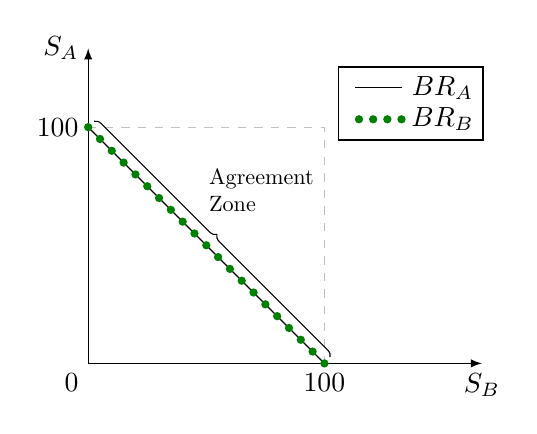
\begin{tikzpicture}[>=latex,
		circ/.pic={\fill[green!50!black] (0,0) circle(1.5pt);}]
		\draw (0,3)--(3,0);
		\draw[<->] (0,4)--(0,0)--(5,0);
		\draw[dashed,lightgray] (0,3)-|(3,0);
		\draw[decoration={brace,raise=3pt},decorate]
		(0,3)--(3,0);
		\foreach \i in {0,.05,...,1.05}
		\path (0,3)--(3,0) pic[pos=\i]{circ};
		\path
		(0,3) node[left]{$100$}
		(3,0) node[below]{$100$}
		(0,0) node[below left]{0}
		(5,0) node[below]{$S_{B}$}
		(0,4) node[left]{$S_{A}$}
		(2.2,2.2) node[align=left,scale=.8] {Agreement\\Zone};
		% for legend
		\begin{scope}[local bounding box=L,shift={(4.5,3.5)}]
			\path (0,0) node (A) {$BR_A$}
			(-90:.4) node (B) {$BR_B$};
			\draw (A.west)--+(180:.6);
			\foreach \i in {0,.3,...,1}
			\path (B.west)--+(180:.6) pic[pos=\i]{circ};
		\end{scope}
		\draw ([xshift=-2mm]L.south west) rectangle (L.north east);
	\end{tikzpicture}
	%\end{figure}
\end{document}